\documentclass[xetex,table]{beamer}

\usepackage{fontspec}
\usepackage[autostyle]{csquotes}
\usepackage{hyperref}
\usepackage{color}
\usepackage{setspace}
\usepackage{listings}
\usepackage{minted}

\usetheme{Pittsburgh}
\usecolortheme{beaver}

\usemintedstyle{perldoc}

\title{How I survived to a SoC with a terrible Linux BSP}
\subtitle{Jurassic vendor kernels, missing pieces and buggy code}
\author{Luca Ceresoli\\
  \href{mailto:luca@lucaceresoli.net}{luca@lucaceresoli.net}\\
  \url{http://lucaceresoli.net}
}
\date{FOSDEM 2017}

\AtBeginSection[]
{
  \begin{frame}{}
    \huge
    \begin{center}
      \insertsection
    \end{center}
  \end{frame}
}

\begin{document}

\maketitle

\begin{frame}{About me}
  \begin{itemize}
  \item Open source enthusiast
    \begin{itemize}
    \item Contributor to Buildroot and a few other projects
    \end{itemize}
  \item Embedded Linux engineer
    \begin{itemize}
    \item Develop real products on custom hardware
    \item Kernel, bootloader, drivers
    \item Integration, build system
    \end{itemize}
  \end{itemize}
\end{frame}

\section{Introduction}

\begin{frame}{Typical embedded Linux system}
  \begin{itemize}
  \item A physical product
    \begin{itemize}
    \item based on an ad-hoc electronic board
    \item Built around a System-on-Chip (SoC)
    \end{itemize}
  \end{itemize}
\end{frame}

\begin{frame}{The System on Chip}
  \begin{itemize}
  \item Nuvoton N32926
    \begin{itemize}
    \item Cheap
    \item ARM926EJ-S @ 240 MHz
    \item Peripherals: H.264 en/decoder, Ethernet MAC, USB, CMOS
      sensor interface, video out, LCD controller, sound, \dots
    \item 64 MB DDR2 {\em on package}
    \item LQFP package
    \end{itemize}
  \item{\tiny Source:
    \url{https://www.nuvoton.com/hq/products/microprocessors/arm9-mpus/n3292-h.264-codec-series/n32926u1dn}}
  \end{itemize}
\end{frame}

\begin{frame}{The ideal BSP}
  \begin{itemize}
  \item BSP = Board Support Package
  \item The ideal BSP
    \begin{itemize}
    \item Mainline kernel
    \item Mainline U-Boot or Barebox
    \item Good hardware documentation
    \end{itemize}
  \item Why?
    \begin{itemize}
    \item All standard, open-source components
      \begin{itemize}
      \item Well known quality
      \item Community and commercial support
      \item Maintained (bugfixes!)
      \end{itemize}
    \item Reuse components
      \begin{itemize}
      \item Infrastructure from other products
      \item Any open source package (including those on your PC)
      \end{itemize}
    \end{itemize}
  \end{itemize}
\end{frame}

\section{The Quest}

\begin{frame}{The quest}
  \begin{itemize}
  \item Documentation
  \item Linux kernel
  \item Toolchain
  \item Booting
  \item Tools
  \item Customer support
  \end{itemize}
\end{frame}

\section{Documentation}

\begin{frame}{Public documentation}
  \begin{itemize}
  \item Website:{\tiny
    \url{https://www.nuvoton.com/hq/products/microprocessors/arm9-mpus/n3292-h.264-codec-series/n32926u1dn}}
  \item An 8-page datasheet (mostly a list of features)
  \end{itemize}
\end{frame}

\begin{frame}{Documentation for customers}
  \begin{itemize}
  \item Only under NDA
  \end{itemize}
\end{frame}

\begin{frame}{Accessible documentation}
  \begin{itemize}
  \item A ``low-cost'' devkit is available from chinese online stores
  \item Contains a DVD-ROM with a subset of the BSP for customers
    \begin{itemize}
    \item Documentation and software
    \item Contains the N3292x Design Guide
      \begin{itemize}
      \item SoC peripherals (registers)
      \end{itemize}
    \end{itemize}
  \end{itemize}
  \begin{center}
    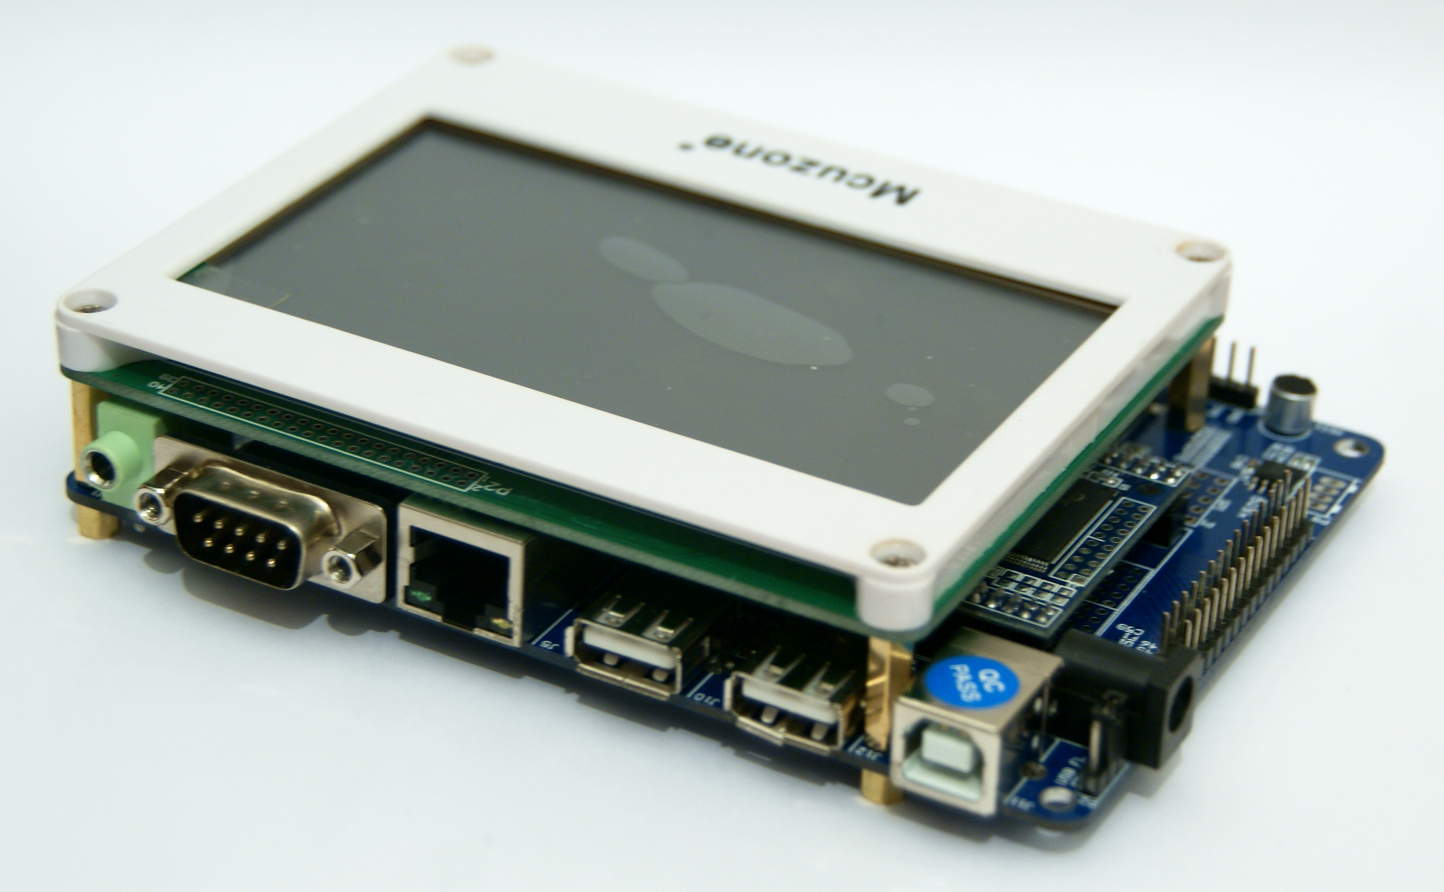
\includegraphics[height=0.4\textheight]{images/devkit.jpg}
  \end{center}
\end{frame}

\section{Linux kernel}

\begin{frame}{Vendor kernel VS mainline kernel}
  \begin{itemize}
  \item Linux 2.6.35.4 (2010)
  \item Delta from the latest 2.6.35.y (v2.6.35.14)
    \begin{itemize}
    \item 11 months, 1382 bugfix commits
    \item Merging them has minimal conflicts
    \end{itemize}
  \item Delta from the latest mainline release
    \begin{itemize}
    \item A countless number of bugfixes, performance improvements, new features
    \item Security
    \item Device Tree
    \end{itemize}
  \end{itemize}
\end{frame}

\begin{frame}{Vendor kernel additions}
  \begin{itemize}
  \item Provided as patches:
    \begin{itemize}
    \item \texttt{w55fa92-kernel-2.6.35-000.patch} (3.6 MB)
    \item \texttt{w55fa92-kernel-2.6.35-001.patch} (1.4 MB)
    \item \texttt{w55fa92-kernel-2.6.35-002.patch} (0.4 MB)
    \item \texttt{do\_kernel\_patch.sh}
    \end{itemize}
  \item Total: 170.000 lines changed
  \end{itemize}
\end{frame}

\begin{frame}{Vendor kernel issues}
  \begin{enumerate}
  \item Bugs
  \item Missing features
  \item Code quality
  \end{enumerate}
\end{frame}

\begin{frame}{Bugs}
  Examples:
  \begin{itemize}
  \item Sound Processing Unit ALSA driver
    \begin{itemize}
    \item \texttt{arecord myfile.wav} \textrightarrow{} kernel crash
      \begin{itemize}
      \item \texttt{NULL} pointer dereference
      \end{itemize}
    \end{itemize}
  \item H.264 decoder driver
    \begin{itemize}
    \item Works with sample streams
    \item Kernel crash on streaming packet loss
      \begin{itemize}
      \item Several \texttt{NULL} pointer dereferences
      \end{itemize}
    \end{itemize}
  \end{itemize}
\end{frame}

\begin{frame}{Missing features}
  Examples:
  \begin{itemize}
  \item GPIO
    \begin{itemize}
    \item Basic functionality is implemented
    \item No interrupt handling
    \end{itemize}
  \item Power Management
    \begin{itemize}
    \item Implemented with a proprietary API
    \item Also implemented the Linux standard way, but incomplete and
      not working
    \end{itemize}
  \end{itemize}
\end{frame}

\begin{frame}{Code quality}
  \begin{itemize}
  \item Average quality of additions: generally bad
  \item Trivial metric: +521 lines starting with \texttt{\#if 0}
  \item A few examples follow
  \end{itemize}
\end{frame}

\begin{frame}[fragile]{Code quality /1}
  Changes to \texttt{Makefile}:

  \begin{minted}[fontsize=\scriptsize]{diff}
-ARCH?= $(SUBARCH)
-CROSS_COMPILE?=
-CROSS_COMPILE?= $(CONFIG_CROSS_COMPILE:''%''=%)
+#ARCH?= $(SUBARCH)
+ARCH= arm
+#CROSS_COMPILE?=
+#CROSS_COMPILE?= $(CONFIG_CROSS_COMPILE:''%''=%)
+CROSS_COMPILE= arm-linux-
  \end{minted}

  \begin{itemize}
  \item Prevents using toolchains with a different prefix
  \item Any advantage?
  \end{itemize}
\end{frame}

\begin{frame}[fragile]{Code quality /2}
  Changes to \texttt{arch/arm/boot/Makefile}:

  \begin{minted}[fontsize=\scriptsize]{udiff}
 $(obj)/Image: vmlinux FORCE
         $(call if_changed,objcopy)
         @echo '  Kernel: $@ is ready'

+ifeq ($(CONFIG_ARCH_W55FA92),y)
+        cp $@   ../image/conprog.bin
+endif
  \end{minted}

  \begin{itemize}
  \item \texttt{../image/} does not make sense in any buildsystem
  \end{itemize}
\end{frame}

\begin{frame}[fragile]{Code quality /3}
  \texttt{sound/soc/w55fa92/w55fa92\_spu.c}:

  \begin{minted}[fontsize=\scriptsize]{c}
    if (nChannels ==1)
    {
        DrvSPU_EnableInt(_u8Channel0, DRVSPU_ENDADDRESS_INT);
        DrvSPU_EnableInt(_u8Channel0, DRVSPU_THADDRESS_INT);
    }
    else
    {    /* just open one channel interrupt */
        DrvSPU_EnableInt(_u8Channel0, DRVSPU_ENDADDRESS_INT);
        DrvSPU_EnableInt(_u8Channel0, DRVSPU_THADDRESS_INT);
    }
  \end{minted}

  \begin{itemize}
  \item Find the differences between the {\em then} and the {\em else} branch
  \end{itemize}
\end{frame}

\begin{frame}[fragile]{Code quality /4}
  \texttt{sound/soc/w55fa92/w55fa92\_spu.c}:

  \begin{minted}[fontsize=\scriptsize]{c}
static int DrvSPU_EnableInt(u32 u32Channel, u32 u32InterruptFlag)
{
  if ( (u32Channel >=eDRVSPU_CHANNEL_0) && (u32Channel <=eDRVSPU_CHANNEL_31) )
  {
    /* ... */
    if (u32InterruptFlag & DRVSPU_USER_INT)
    {
      AUDIO_WRITE(REG_SPU_CH_EVENT, AUDIO_READ(REG_SPU_CH_EVENT) | EV_USR_EN);
    }
    if (u32InterruptFlag & DRVSPU_SILENT_INT)
    {
      AUDIO_WRITE(REG_SPU_CH_EVENT, AUDIO_READ(REG_SPU_CH_EVENT) | EV_SLN_EN);
    }
    /* ...a few more times... */

    /* ... */
    return E_SUCCESS;
  }
  else
    return E_DRVSPU_WRONG_CHANNEL;
}
  \end{minted}
\end{frame}

\begin{frame}[fragile]{Code quality /5}
  \texttt{arch/arm/mach-w55fa92/include/mach/w55fa92\_gpio.h}:

  \begin{minted}[fontsize=\scriptsize]{c}
static inline int w55fa92_gpio_configure(int group, int num) {
  /* ... */
    case GPIO_GROUP_B:
      if(num <= 7)
        writel(readl(REG_GPBFUN0) &~ (0xF << (num<<2)), REG_GPBFUN0);
      else
        writel(readl(REG_GPBFUN1) &~ (0xF << ((num%8)<<2)), REG_GPBFUN1);
      break;

    case GPIO_GROUP_C:
      if(num <= 7)
        writel(readl(REG_GPCFUN0) &~ (0xF << (num<<2)), REG_GPCFUN0);
      else
        writel(readl(REG_GPCFUN1) &~ (0xF << ((num%8)<<2)), REG_GPCFUN1);
      break;
  /* ...similarly fo other GPIO ports... */
}
  \end{minted}

  \begin{itemize}
  \item A little refactoring would help
  \end{itemize}
\end{frame}

\begin{frame}[fragile]{Code quality: driver model}
  \texttt{drivers/video/w55fa92\_fb.c}:

  \begin{minted}[fontsize=\scriptsize]{c}
#ifdef  CONFIG_GIANTPLUS_GPM1006D0_320X240
#include "w55fa92_GIANTPLUS_GPM1006D0.c"
#endif

#ifdef  CONFIG_TOPPLY_320X240
#include "w55fa92_TOPPLY_320x240.c"
#endif

/* ...5 more displays... */

#if 0
  #ifdef  CONFIG_SHARP_LQ035Q1DH02_320X240
  #include "w55fa92_Sharp_LQ035Q1DH02.c"
  #endif

  #ifdef  CONFIG_WINTEK_WMF3324_320X240
  #include "w55fa92_Wintek_WMF3324.c"
  #endif

  /* ...5 more displays... */
#endif
  \end{minted}
\end{frame}

\begin{frame}[fragile]{Code quality: H.264 codec memory allocation}
  \texttt{drivers/misc/codec264/favc\_module.c}:

  \begin{minted}[fontsize=\scriptsize]{c}
unsigned int get_avc_buffer_size(void)
{
  /* ...~90 lines... */
  return TOTAL_VDE_BUF_SIZE;
}
EXPORT_SYMBOL(get_avc_buffer_size);
  \end{minted}

  From {\small\texttt{arch/arm/mm/mmu.c}}:
  \begin{minted}[fontsize=\scriptsize]{c}
extern unsigned int get_avc_buffer_size(void);
void __init reserve_node_zero(pg_data_t *pgdat)
{
  /* ... */
  buffer_size = get_avc_buffer_size();
  printk("AVC Buffer Size: 0x%x\n",buffer_size);
  w55fa92_vde_v = alloc_bootmem_low_pages (buffer_size);
  /* ... */
}
  \end{minted}
\end{frame}

\section{Toolchain}

\begin{frame}{Vendor toolchain}
  \begin{itemize}
  \item The BSP provides a toolchain.
    \begin{itemize}
    \item Why?
    \end{itemize}
  \item What's inside
    \begin{itemize}
    \item gcc 4.2.1 (July 2007)
      \begin{itemize}
      \item No C++11 support
      \item gcc 4.2.x got fixes until 4.2.4 (May 2008)
      \end{itemize}
    \item uClibc 0.9.29 (2007)
      \begin{itemize}
      \item What if I need glibc or musl?
      \item Bugfixes and improvements in later versions?
      \end{itemize}
    \item A few other libraries (libcurl, libpng \dots)
    \item A hand-crafted script to install it at a hard-coded location
    \end{itemize}
  \end{itemize}
\end{frame}

\begin{frame}{Toolchain selection}
  \begin{itemize}
  \item Don't use the provided toolchain
  \item You could use a pre-built toolchain
    \begin{itemize}
    \item If it has been built with kernel headers <= 2.6.35
    \item So it's probably quite old itself
    \end{itemize}
  \item Build you own
    \begin{itemize}
    \item crosstool-NG, Buildroot, Openembedded\dots
    \end{itemize}
  \end{itemize}
\end{frame}

\section{Booting}

\begin{frame}{Bootloaders in the BSP}
  \begin{itemize}
  \item No U-Boot
  \item No Barebox
  \item Some proprietary bootloaders
    \begin{itemize}
    \item Sources provided
    \item Not open source
    \end{itemize}
  \end{itemize}
\end{frame}

\begin{frame}{Vendor booting scheme (NAND)}
  \begin{center}
    \includegraphics[width=1.0\textwidth]{images/booting.pdf}
  \end{center}
\end{frame}

\begin{frame}{Vendor booting scheme pros}
  \begin{itemize}
  \item Easy deployment of demos provided by vendor
    \begin{enumerate}
    \item Press  a button during boot
    \item Mount mass storage on PC
    \item Replace files
    \end{enumerate}
  \end{itemize}
\end{frame}

\begin{frame}{Vendor booting scheme issues /1}
  \begin{itemize}
  \item FAT
    \begin{itemize}
    \item Unreliable on power loss
    \item It just cannot contain a UNIX-like rootfs (no users, groups,
      permissions, symlinks...)
    \end{itemize}
  \item NAND FTL
    \begin{itemize}
    \item FAT-on-NAND emulation (with FTL) is in a binary module
    \item NVT Loader cannot mount UBIFS
  \end{itemize}
  \item No provision for redundancy: one copy of each component
  \end{itemize}
\end{frame}

\begin{frame}{Vendor booting scheme issues /2}
  \begin{itemize}
  \item Root filesystem is an initramfs
    \begin{itemize}
    \item Changes are volatile
    \item Limited size, everything in RAM
    \item Persistent changes stay in FAT
    \end{itemize}
  \item Nobody passes cmdline to kernel
    \begin{itemize}
    \item it must be hard-coded in the kernel (\texttt{CONFIG\_CMDLINE})
    \end{itemize}
  \item NFS booting
    \begin{itemize}
    \item Needs cmdline parameters \textrightarrow{} must rebuild and
      reflash the kernel
    \end{itemize}
  \item Cannot load kernel via TFTP
  \end{itemize}
\end{frame}

\begin{frame}
  \begin{center}
    Alternative booting options?
  \end{center}
\end{frame}

\begin{frame}{Option 1: add a SquashFS layer on top of FAT}
  \begin{center}
    \includegraphics[width=1.0\textwidth]{images/booting-on-fat.pdf}
  \end{center}
  \begin{itemize}
  \item Keep the existing structure untouched
  \item Remove FAT space constraint and RAM usage
  \item Still read-only
    \begin{itemize}
    \item ext2 or any other rw filesystem over FAT over NAND is crazy
    \end{itemize}
  \item The device cannot atomically upgrade itself
  \end{itemize}
\end{frame}

\begin{frame}{Option 2: jump from FAT to UBIFS}
  \begin{center}
    \includegraphics[width=1.0\textwidth]{images/booting-fat-ubi.pdf}
  \end{center}
  \begin{itemize}
  \item UBI and UBIFS are designed for NAND! (efficient, reliable, quite scalable)
  \item Tweaks needed
    \begin{itemize}
    \item Change the initramfs \texttt{/init} to mount UBIFS and \texttt{switch\_root}
    \item Tweak NVT Loader not to use all space for FAT
    \end{itemize}
  \item USB mass storage can only update kernel
  \item FAT area atrophied, NVT Loader almost useless
  \end{itemize}
\end{frame}

\begin{frame}{Option 3: skip NVT Loader}
  \begin{center}
    \includegraphics[width=1.0\textwidth]{images/booting-no-nvt-loader.pdf}
  \end{center}
  \begin{itemize}
  \item NAND Loader loads kernel \texttt{Image} to address \texttt{0} and jump there
  \item No more NVT Loader and FAT
    \begin{itemize}
    \item Less code, less bugs, faster boot, more free space
    \end{itemize}
  \item Kernel still on bare NAND and without cmdline
  \item Safe kernel upgrade?
    \begin{itemize}
    \item kexec
    \end{itemize}
  \end{itemize}
\end{frame}

\begin{frame}{Option 4: Port U-Boot}
  \begin{itemize}
  \item Port U-Boot or Barebox to the SoC
    \begin{itemize}
    \item Maybe keeping the vendor NAND Loader (SPL)
    \end{itemize}
  \item Unleashes all the known advantages
    \begin{itemize}
    \item Environment, boot-time scripting, prompt, cmdline, TFTP boot\dots
    \item Redundancy for all/most components on bare NAND
    \end{itemize}
  \item Time to market?
  \end{itemize}
\end{frame}

\section{Tools}

\begin{frame}{Tools}
  \begin{itemize}
  \item Which tools do I need?
    \begin{itemize}
    \item Ideally, none
    \end{itemize}
  \item Flashing an empty memory is different
    \begin{itemize}
    \item Some vendors have proprietary tools
    \end{itemize}
  \end{itemize}
\end{frame}

\begin{frame}{Flashing tools}
  \begin{itemize}
  \item Tool provided to write memory
  \item Quite flexible
    \begin{itemize}
    \item Can write NAND, SPI, SD, SDRAM (and execute)
    \item Over USB
    \end{itemize}
  \item For Windows only
  \item Proprietary
  \item GUI, not scriptable
  \item Protocol to Boot ROM not documented
  \item[\textrightarrow] You're locked to it
  \end{itemize}
\end{frame}

\begin{frame}{NAND partition table}
  \begin{columns}
    \column{0.6\textwidth}
    \begin{itemize}
    \item Proprietary partition table in the NAND Loader area
    \item The proprietary tool writes only this format
    \item Not a bad idea
      \begin{itemize}
        \item but standard tools work differently
    \end{itemize}
    \item[\textrightarrow] You can't get rid of the table
    \end{itemize}
    \column{0.4\textwidth}
    \includegraphics[width=\textwidth]{images/pseudo-partition-table.pdf}
  \end{columns}
\end{frame}

\section{Customer support}

\begin{frame}{Customer support}
  \begin{itemize}
  \item Standard, mainline code
    \begin{itemize}
    \item Plenty of options for community and commercial support
    \end{itemize}
  \item Proprietary code with sources
    \begin{itemize}
    \item Vendor support
    \item Read the code
    \end{itemize}
  \item Proprietary, binary software (and hardware issues)
    \begin{itemize}
    \item One choice: vendor support
    \item Still acceptable if support is good
      \begin{itemize}
        \item But don't bet it will be
      \end{itemize}
    \end{itemize}
  \end{itemize}
\end{frame}

\begin{frame}{Customer support issues}
  \begin{itemize}
  \item The engineer who knows the answer is hidden by reseller
    sales dept., FAE, customer support department
  \item Responsiveness
  \item Timezone issues
  \end{itemize}
\end{frame}

\begin{frame}{Customer support --- a bad example}
  A real conversation (short form)
  \begin{description}
  \item[Me] The proprietary tool doesn't work
  \item[CS] Works on my PC, see screenshot
  \item[Me] Not on mine; can it log errors so you can diagnose it?
  \item[CS] Adding logging would not be practical
  \end{description}
\end{frame}

\section{Concluding remarks}

\begin{frame}{The result}
  Comparison with a well-supported SoC
  \begin{itemize}
  \item The product works
    \begin{itemize}
    \item Final quality is lower
    \item The hardware would allow to do better
    \end{itemize}
  \item Extra time spent
    \begin{itemize}
    \item Sometimes we supported ourselves
    \item Look for stuff in the BSP
    \item Fix bugs
    \item Reinvent booting
    \end{itemize}
  \end{itemize}
\end{frame}

\begin{frame}{What can I do to improve things?}
  What can I do to make a better world?
  \begin{itemize}
  \item As an embedded Linux engineer
    \begin{itemize}
    \item Assess potential problem early while evaluating a SoC
      \begin{itemize}
      \item Especially booting and hardware support
      \end{itemize}
    \end{itemize}
  \item As a hobbyist or a hacker
    \begin{itemize}
    \item Pick boards with good mainline support, or\dots
    \item Improve existing support and mainline it
    \end{itemize}
  \end{itemize}
\end{frame}

\begin{frame}{What can vendors do to ship better BSPs?}
  \begin{itemize}
  \item Happy engineer = good product = more sales
  \item Don't reinvent the wheel
  \item Write good docs, no NDA, no registration
    \begin{itemize}
    \item Including yout Boot ROM protocol
      \begin{itemize}
      \item And let people write the tools they want
      \end{itemize}
    \end{itemize}
  \item Push your code to mainline\\
    {\small (or outsource this to a specialized company)}
    \begin{itemize}
    \item Expensive, but rewarding
    \item Somebody else will update, fix, improve and support it
    \end{itemize}
  \item Leverage the community
    \begin{itemize}
    \item Let your engineers use mailing-lists, IRC etc
    \item Make cheap, hacker-friendly boards
    \end{itemize}
  \end{itemize}
\end{frame}

\begin{frame}
  \begin{center}
    Thank you for your attention

    \vspace{0.15\textheight}

    {\Huge Questions?}

    \vspace{0.15\textheight}

    \href{mailto:luca@lucaceresoli.net}{luca@lucaceresoli.net}\\
    \url{http://lucaceresoli.net}

    \textcopyright{} Copyright 2017, Luca Ceresoli\\

    \vspace{0.05\textheight}

    \tiny
    Slides released under\\
    Creative Commons Attribution - Share Alike 3.0 License \\
    \url{https://creativecommons.org/licenses/by-sa/3.0/} \\
\end{center}
\end{frame}

\section{Extra Slides}

\begin{frame}[fragile]{Using an old gcc --- an example}
  A C++ program using libconfuse 3.0

  \begin{minted}[fontsize=\scriptsize]{c++}
    #include <confuse.h>
    //...
    cfg_opt_t opts[] =
    {
      CFG_STR("my-param", "defval", CFGF_NONE),
      CFG_END()
    };
  \end{minted}

  With gcc <= 4.8 fails building due to designated initializers not being implemented:

  \texttt{ error: expected primary-expression before '.' token}
\end{frame}

\end{document}
